\documentclass{article}
\usepackage[left=3cm,right=3cm,top=2cm,bottom=2cm]{geometry} % page settings
\usepackage{amsmath} % provides many mathematical environments & tools
\usepackage{graphicx}
\usepackage{mathrsfs}
\usepackage{amssymb}
\usepackage{algorithm}
\usepackage[noend]{algpseudocode}
\usepackage{mathtools}
\usepackage{textcomp}

\setlength{\parindent}{0mm}
\makeatletter
\setlength{\@fptop}{0pt}
\makeatother
\def\BState{\State\hskip-\ALG@thistlm}

\newcommand{\RNum}[1]{\uppercase\expandafter{\romannumeral #1\relax}}
\DeclarePairedDelimiter\ceil{\lceil}{\rceil}
\DeclarePairedDelimiter\floor{\lfloor}{\rfloor}


\begin{document}

\title{CSE 250A: Assignment 4}
\author{Jiaxu Zhu~~A53094655}
\date{\today}
\maketitle
%%%%%%%%%%%%%%%%%%%%%%%%%%%%%%%%%%%%%%%%%%%%%%%%%%%%%%%%%%%%%%%%%%%%%%%%%%%%%%%%%%%%%%%%%%%
\subsection*{4.1 Gradient-based learning}
\subparagraph*{(a)}
\begin{eqnarray*}
	P(y_t|⃗\vec{x}_t) &=& p_t^{y_t} + (1-p_t)^{1-y_t} \\
	\mathcal{L} &=& \sum_{t=1}^{T}\log P(y_t|⃗\vec{x}_t) \\
	&=&\sum_{t=1}^{T}[y_t\log p_t + (1-y_t)\log (1-p_t)]\\
	\frac{\partial \mathcal{L}}{\partial w_i}	
	&=& \sum_{t=1}^{T} y_t \frac{x_{it}f'(\vec{w} \cdot \vec{x}_t)}{p_t} - (1 - y_t) \frac{x_{it}f'(\vec{w} \cdot \vec{x}_t)}{1-p_t}\\
	&=& \sum_{t=1}^{T} f'(\vec{w} \cdot \vec{x}_t) \frac{y_t - p_t}{p_t(1-p_t)} x_{it}\\
	&=& \sum_{t=1}^{T} \left[\frac{f'(\vec{w} \cdot \vec{x}_t)}{p_t(1-p_t)}\right](y_t - p_t)x_{it}
\end{eqnarray*}

\subparagraph*{(b)}
\begin{eqnarray*}
	f'(z) &=& \frac{e^{-z}}{(1+e^{-z})^2}\\
	p_t &=& \frac{1}{1+e^{-\vec{w} \cdot \vec{x}_t}}\\
	\frac{\partial \mathcal{L}}{\partial w_i} &=& \sum_{t=1}^{T}\left[\frac{\frac{e^{-\vec{w} \cdot \vec{x}_t}}{(1+e^{-\vec{w} \cdot \vec{x}_t})^2}}{\frac{e^{-\vec{w} \cdot \vec{x}_t}}{(1+e^{-\vec{w} \cdot \vec{x}_t})^2}}\right](y_t - p_t)x_{it}\\
	&=&\sum_{t=1}^{T}(y_t - p_t)x_{it}
\end{eqnarray*}

\subsection*{4.2 Multinomial logistic regression}

\begin{eqnarray*}
	P(y_t|⃗\vec{x}_t) &=& \sum_{k=1}^{c}p_{kt}^{y_{kt}} + (1-p_{kt})^{1-y_{kt}}\\
	\mathcal{L} &=& \sum_{t=1}^{T}\log P(y_t|⃗\vec{x}_t) \\
	&=&\sum_{t=1}^{T}\sum_{k=1}^{c}[y_{kt}\log p_{kt} + (1-y_{kt})\log (1-p_{kt})]\\
	\frac{\partial \mathcal{L}}{\partial \vec{w}_i} &=&
	\sum_{t=1}^{T} \frac{y_{it}}{p_{it}} \frac{\partial p_{it}}{\partial \vec{w}_i} - \frac{1-y_{it}}{1-p_{it}} \frac{\partial p_{it}}{\partial \vec{w}_i}\\
	&=&\sum_{t=1}^{T} \left[\frac{y_{it} - p_{it}}{p_{it}(1-p_{it})}\right]\frac{\partial p_{it}}{\partial \vec{w}_i}\\
	p_{it}(1-p_{it}) &=& \frac{e^{\vec{w}_i \cdot \vec{x}_t}(\sum_{j=1}^{c}e^{\vec{w}_j \cdot \vec{x}_t} - e^{\vec{w}_i \cdot \vec{x}_t})}{(\sum_{j=1}^{c}e^{\vec{w}_j \cdot \vec{x}_t})^2}\\
	\frac{\partial p_{it}}{\partial \vec{w}_i} &=& \frac{e^{\vec{w}_i \cdot \vec{x}_t}(\sum_{j=1}^{c}e^{\vec{w}_j \cdot \vec{x}_t} - e^{\vec{w}_i \cdot \vec{x}_t})}{(\sum_{j=1}^{c}e^{\vec{w}_j \cdot \vec{x}_t})^2} \vec{x}_t\\
	\frac{\partial \mathcal{L}}{\partial \vec{w}_i} &=&\sum_{t=1}^{T}(y_{it} - p_{it})\vec{x}_{t}
\end{eqnarray*}

\subsection*{4.3 Convergence of gradient descent}
\subparagraph*{(a)}
\begin{eqnarray*}
	f'(x) &=& \alpha (x-x_{\star})\\
	&=& \alpha \varepsilon\\
	x_{n+1} &=& x_n - \eta \alpha \varepsilon_n\\
	\varepsilon_{n+1} &=& (1-\eta\alpha)\varepsilon_n\\
	&=& (1-\eta\alpha)^n \varepsilon_0\\	
\end{eqnarray*}

\subparagraph*{(b)}
In order to converge to the minimum
\begin{eqnarray*}
|(1-\eta\alpha)| &<& 1\\
 0 < \eta &<& \frac{2}{\alpha}
\end{eqnarray*}
As we can see, $\varepsilon_n$ cannot really reach 0 except one situation
\begin{eqnarray*}
	(1-\eta'\alpha) &=& 0\\
	\eta' &=& \frac{1}{\alpha}
\end{eqnarray*} 
while $f''(x_n) = \alpha$, we can say that $\eta' = \frac{1}{f''(x_n)}$
\subparagraph*{(c)}
\begin{eqnarray*}
	x_{n+1} &=& x_n - \eta \alpha \varepsilon_n + \beta(x_n - x_{n-1})\\
	x_{n+1}-x_{\star} &=& (x_n - x_{\star}) - \eta \alpha \varepsilon_n + \beta[(x_n-x_{\star}) - (x_{n-1}-x_{\star})]\\
	\varepsilon_{n+1} &=& (1-\eta\alpha + \beta)\varepsilon_n - \beta \varepsilon_{n-1}\\
\end{eqnarray*}

\subparagraph*{(d)}
for $\eta = \frac{4}{9}, \beta = \frac{1}{9}$,
\begin{eqnarray*}
	\varepsilon_{n+1} &=& \frac{2}{3}\varepsilon_n - \frac{1}{9} \varepsilon_{n-1}\\
\end{eqnarray*}

assume that $\varepsilon_n = \lambda^n \varepsilon_0$
\begin{eqnarray*}
	\lambda^{n+1} \varepsilon_0 &=& \frac{2}{3}\lambda^n\varepsilon_0 - \frac{1}{1} \lambda^{n-1} \varepsilon_0\\
	9\lambda^2 - 6\lambda + 1 &=& 0\\
	\lambda &=& \frac{1}{3}\\
	\varepsilon_n &=& \frac{1}{3}^n \varepsilon_0
\end{eqnarray*}
for $\eta = \frac{4}{9}, \beta = 0$, we have $\varepsilon_{n+1} = \left(\frac{5}{9}\right)^n\varepsilon_0$, this rate of convergence compare to that of gradient descent with the
same learning rate is fast than $\eta = \frac{4}{9}, \beta = \frac{1}{9}$.

\subsection*{4.4 Newton’s method}
\subparagraph*{(a)}
\begin{eqnarray*}
	f'(x)&=&2p(x-x_{\star})^{2p-1}\\
	f''(x)&=&2p(2p-1)(x-x_{\star})^{2p-2}\\
	x_{n+1}&=& x_{n} - \frac{f'(x_n)}{f''(x_n)}\\
	&=&x_n - \frac{1}{2p-1}(x_n-x_{\star})\\
	x_{n+1} - x_{\star} &=&   \frac{2p-2}{2p-1} (x_{n} - x_{\star})\\
	\varepsilon_{n+1} &=& \frac{2p-2}{2p-1} \varepsilon_n\\
	\varepsilon_n &=& \left(\frac{2p-2}{2p-1}\right)^n \varepsilon_0
\end{eqnarray*}

\subparagraph*{(b)}
\begin{eqnarray*}
	\varepsilon_n &\le& \sigma \varepsilon_0\\
	\left(\frac{2p-2}{2p-1}\right)^n &\le& \sigma\\
	n\log\left(\frac{2p-2}{2p-1}\right) &\le& \log(\sigma)\\
	n(\frac{2p-2}{2p-1}-1) &\le& \log(\sigma)\\
	n(\frac{-1}{2p-1}) &\le& \log(\sigma)\\\
	n &\ge& -(2p-1)\log(\sigma) = (2p-1)\log(\frac{1}{\sigma})
\end{eqnarray*}

\subparagraph*{(c)}
\begin{eqnarray*}
	f'(x) &=& x_{\star} \frac{x}{x_{\star}} x_{\star} \frac{-1}{x^2} + 1\\
	&=& -\frac{x_{\star}}{x} + 1\\
	f''(x) &=& \frac{x_{\star}}{x^2}\\
\end{eqnarray*}
let $f'(x)=0$, we have $x = x_{\star}$, and also $f''(x)>0$, which means that the minimum occurs at $x = x_{\star}$. The sketch of the function in the region $|x-x_{\star}|<x_{\star}$ is shown in Fig. \ref{hw4.4}.

\begin{figure}
	\centering
	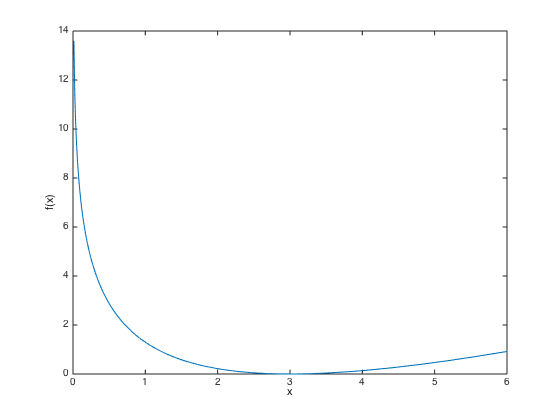
\includegraphics[width=8cm]{hw44.png}
	\caption{The sketch of the function in the region $|x-x_{\star}|<x_{\star}$}
	\label{hw4.4}
\end{figure}
\subparagraph*{(d)}
\begin{eqnarray*}
	x_{n+1}&=& x_{n} - \frac{f'(x_n)}{f''(x_n)}\\
	&=&  - \frac{x_n^2-2x_n x_{\star}}{x_{\star}}\\
	\frac{x_{n+1-x_{\star}}}{x_{\star}} &=& - \left(\frac{x_n - x_{\star}}{x_{\star}}\right)^2\\
	\rho_{n+1} &=& -\rho_n^2
\end{eqnarray*}

if you want Newton’s method converge to the correct answer, you should have $|\rho_0| < 1$

\begin{eqnarray*}
	|\rho_0| &<& 1\\
	|\frac{x_0 - x_{\star}}{x_{\star}}| &<& 1\\
	0 &<& x_0 < 2x_{\star}
\end{eqnarray*}

\subsection*{4.5 Stock market prediction}
\subparagraph*{(a)}
$(a_1,a_2,a_3) = (0.9368, 0.0421, 0.0193)$
\subparagraph*{(b)}
The mean square error is 13907.7327964 for training data and 2995.03281029 testing data, which are relatively big errors. It means that this linear model would not be recommended for stock market prediction.

\subsection*{4.6 Handwritten digit classification}
\subparagraph*{(a)}
we trained two models to classify if this digit is 3 and if this digit is 5. Thus we have two set of weights. Fig. \ref{converge} shows that the log-likelihood of two models have all converged after 2500 iterations (the upper one is 3-model). the error rate for training data is $4\%$, and the learned weight is:

\begin{eqnarray*}
	\vec{w}_3 &=& \left[ \begin{array}{cccccccc}
		0.8395 & 0.9865 & 1.2490 & 0.8981 & 1.1110 & 0.2113 & -0.8863 & -1.5580 \\
		-0.2841 & -0.1960 & -0.3359 & 0.2561 & -0.0193 & -0.4072 & 0.8292 & 0.4357 \\
		-1.7249 & -1.0790 & -0.9900 & -0.4671 & -0.1654 & 1.4738 & 2.5408 & 2.3267 \\
		-1.4252 & -0.7379 & -0.8551 & 0.3142 & 0.9042 & 0.5223 & -0.1621 & 0.1622 \\
		-0.2888 & -0.2445 & -0.0587 & 0.3913 & 0.3400 & 0.3584 & 0.3144 & 0.3649 \\
		-0.7987 & 0.5478 & -0.2413 & -0.5009 & -0.3588 & 0.2702 & 0.1209 & 1.1519 \\
		-0.3237 & -0.0268 & -0.6534 & -0.5795 & -0.0732 & 0.1171 & -0.3591 & 0.9304 \\
		0.0557 & -0.3939 & -0.5579 & -1.3870 & -0.4531 & -0.5704 & 0.1809 & 0.2766 \\
	\end{array}\right]\\
	\vec{w}_5 &=& \left[ \begin{array}{cccccccc}
		-0.8395 & -0.9865 & -1.2490 & -0.8981 & -1.1110 & -0.2113 & 0.8863 & 1.5580 \\
		0.2841 & 0.1960 & 0.3359 & -0.2561 & 0.0193 & 0.4072 & -0.8292 & -0.4357 \\
		1.7249 & 1.0790 & 0.9900 & 0.4671 & 0.1654 & -1.4738 & -2.5408 & -2.3267 \\
		1.4252 & 0.7379 & 0.8551 & -0.3142 & -0.9042 & -0.5223 & 0.1621 & -0.1622 \\
		0.2888 & 0.2445 & 0.0587 & -0.3913 & -0.3400 & -0.3584 & -0.3144 & -0.3649 \\
		0.7987 & -0.5478 & 0.2413 & 0.5009 & 0.3588 & -0.2702 & -0.1209 & -1.1519 \\
		0.3237 & 0.0268 & 0.6534 & 0.5795 & 0.0732 & -0.1171 & 0.3591 & -0.9304 \\
		-0.0557 & 0.3939 & 0.5579 & 1.3870 & 0.4531 & 0.5704 & -0.1809 & -0.2766 \\
	\end{array}\right]
\end{eqnarray*}

\begin{figure}
	\centering
	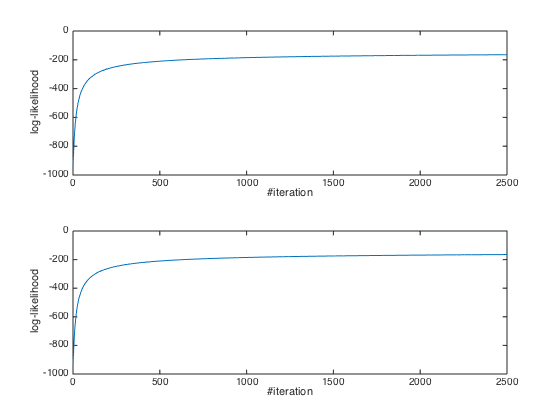
\includegraphics[width=15cm]{converge}
	\caption{The converge of the log-likelihood}
	\label{converge}
\end{figure}

\subparagraph*{(b)}
The error rate on testing data is about $5\%$.
\end{document}

